\documentclass[12pt, openany]{memoir}

\usepackage{graphicx,amsmath}
\usepackage{natbib}
\usepackage{amssymb}
\usepackage{color}
\usepackage{listings}
\usepackage{sidecap}
\usepackage{fancybox}

\chapterstyle{ell}

\newcommand{\degr}{\ensuremath{^\circ}}
\newcommand{\half}{\ensuremath{\frac{1}{2}}}
\newcommand{\pder}[2]{\ensuremath{\frac{\partial #1}{\partial #2}}}
\newcommand{\water}{\ensuremath{{\rm H_2 O\ }}}
\newcommand{\eps}{\dot{\varepsilon}}
\newcommand{\unit}[1]{\ensuremath{\,\mathrm{#1}}}
\newcommand{\cels}[1]{\ensuremath{#1^{\circ}\,\mathrm{C}}}
\newcommand{\norm}[1]{\parallel\! #1\! \parallel}

% -- New Operators --
\DeclareMathOperator{\rot}{rot}
\DeclareMathOperator{\grad}{grad}
\renewcommand{\div}{\text{div}\,}
\DeclareMathOperator{\Tr}{Tr}

\setlength\parindent{0cm}
\begin{document}

\title{CONTINUUM MECHANICS}
\author{Martin Truffer\\ University of Alaska Fairbanks}
\date{2010 McCarthy Summer School}

\maketitle
\pagebreak
\tableofcontents
\pagebreak

\chapter{Introduction}

Continuum mechanics is the application of classical mechanics to
continous media. So,

\begin{itemize}
\item What is Classical mechanics?
\item What are continuous media?
\end{itemize}

\section{Classical mechanics: a very quick summary}

We make the distinction of two types of equations in classical
mechanics: (1) Statements of conservation that are very fundamental to
physics, and (2) Statements of material behavior that are only
somewhat fundamental

\subsection{Conservation Laws}

Statements of physical conservation laws (god-given laws of nature):

\begin{itemize}
\item Conservation of mass
\item Conservation of linear momentum (Newton's Second Law)
\item Conservation of angular momentum
\item Conservation of energy
\end{itemize}

There are other conservation laws (such as those of electric charge),
but these are of no further concern to us right now.

Conservation Laws are good laws. Few sane people would seriously
question them. If your theory/model/measurement does not conserve mass
or energy, you have most likely not discovered a flaw with fundamental physics,
but rather, you should doubt your theory/model/measurement.

We will see that conservation laws are not enough to fully describe a
deforming material. Simply said, there are fewer equations than
unknowns. We also need equations describing material behavior.

\subsection{Material (constitutive) laws}

Material or constitutive laws describe the reaction of a material,
such as ice, to forcings, such as stresses, temperature gradients,
increase in internal energy, application of electric or magnetic
fields, etc. Such "laws" are often empirical (derived from observations rather than fundamental principles) and involve material-dependent "constants". Examples are:

\begin{itemize}
\item Flow law (how does ice deform when stressed?)
\item Fourier's Law of heat conduction (how much energy is transfered across a body of ice, if a temperature difference is applied?)
\end{itemize}

There are other examples that we will not worry about here.

Constitutive laws are not entirely empirical. They have to be such
that they don't violate basic physical principles. Perhaps the most
relevant physical principle here is the Second Law of
Thermodynamics. The material laws have to be constrained, so that heat
cannot spontaneously flow from cold to hot, or heat cannot be turned
entirely into mechanical work. There is a long (and complicated!)
formalism associated with that; we will not be further concerned with
it.

There are other requirements for material laws. The behavior of a
material should not change if the coordinate system is changed
(material objectivity), and any symmetries of the material should be
considered. For example, the ice crystal hexagonal structure implies
certain symmetries that ought to be reflected in a flow law. Here we
assume that ice is isotropic (looks the same from all
directions). This is not always a good assumption (see Erin Pettit's
upcoming lecture).

Conservation laws and constitutive laws constitute the \emph{field
equations}. The field equations together with boundary conditions form
a set of partial differential equations that solve for all the
relevant variables (velocity, pressure, temperature) in an ice
mass. The goal here is to show how we get to these field equations.

\section{Continuous media}

\subsection{Densities}

Classical mechanics has the concept of point mass. We attribute a
finite mass to an infinitely small point. We track the position of the
point and by looking at rates of change of position we determine
velocity and then acceleration. This is known as kinematics. We then
look at how forces affect a point mass or a collection of them (that's
dynamics).

Ice forms a finite sized body of deformable material (a fluid). The challenge
then is to write the laws for point masses such that they apply to
continuous media. To define quantities at a point we introduce the
concept of density. To introduce the density $\rho$, we acknowledge that some
volume $\Omega$ of a fluid has a certain mass $m$. We then write:

\begin{equation}
m = \int_\Omega \rho dv
\end{equation}
Similarly we can define a density for linear momentum:

\begin{equation}
m v = \int_\Omega \rho v dv
\end{equation}
and an internal energy density 

\begin{equation}
U = \int_\Omega \rho u dv 
\end{equation}
We define these quantities somewhat carelessly. In particular, the
concept of density and the mathematical methods of continuum mechanics
imply a mathematical limit process to infinitely small volumes (a
point). This does not make immediate physical sense, as the physical
version of this limit process would go from ice sheet scale to
individual grains, then molecules, atoms, atomic structure, etc. This
would eventually involve physics that is quite different from
classical physics. But we shall not be further concerned with this here.

\subsection{Oh no, tensors!}

The description of continuous media requires the introduction of a new
mathematical creature, the tensor. This is needed to describe forces
in continuous media. Let's cut a little cube out of an ice sheet and
try to see in how many ways we can apply forces to it (see
Figure \ref{fig:tensor}).

\begin{figure*}
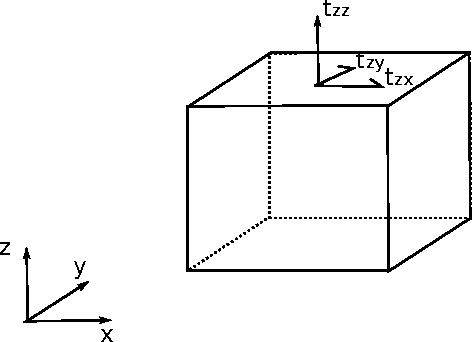
\includegraphics[width=8cm]{tensor}
\caption{\label{fig:tensor} A force applied to the face of a
representative volume can be decomposed into three components}
\end{figure*}

A representative little cube has six faces. Each face can be described
 by a surface normal vector, and each face can be subject
 to a force. A force is a vector quantity, so it has three
 components. We choose one component along the surface normal and
 define it as positive for tension and negative for compression. The
 other two directions are tangential to the face and perpendicular to
 each other. Those are shear forces. In analogy to the definition of
 densities, we know define stresses as forces per unit area. So for
 each face we end up with three stresses. 

Because there are so many faces and force directions we have to agree
on a notation. The stress acting on a face with surface normal $i$ and
in the direction $j$ is written as $t_{ij}$.

There are three principal directions ($x$, $y$, $z$) and each one of
them has a three component force vector associated with it. This
leaves us with nine components of the stress tensor. These nine
components are usually ordered as follows: 

\begin{equation}
\mathbf{t} = \left[ \begin{array}{ccc} t_{xx} & t_{xy} & t_{xz} \\
t_{yx} & t_{yy} & t_{yz} \\ t_{zx} & t_{zy} &
t_{zz} \end{array} \right]
\end{equation}
$t$ is known as the \emph{Cauchy Stress Tensor}. 

A tensor is not just any table of nine numbers. It has some very
special properties that relate to how it changes under a coordinate
transformation. A rotation in 3D can be described by an orthogonal
matrix $R$ with the properties $R=R^T$ and $\det R =1$. A second order
tensor transforms under such a rotation as

\begin{equation}
\mathbf{t'} = \mathbf{R t R}^T
\end{equation}
The way to think about this is that two rotations are involved in this
transformation, one of the face normal, and one of the force vector.

Tensors have quantities associated with it that are invariant under
transformation. A second order tensor has three invariants:
\marginpar{\shadowbox{Invariants}}

\begin{eqnarray}
\mathrm{I}_\mathbf{t} &=& \mathrm{tr} \mathbf{t} \\
\mathrm{II}_\mathbf{t} &=& \frac{1}{2} \left( (\mathrm{tr}\mathbf{t})^2
- \mathrm{tr}( \mathbf{t^2}) \right) \\
\mathrm{III}_\mathbf{t} &=& \det (\mathbf{t})
\end{eqnarray}
Here, tr refers to the trace ($\mathrm{tr} (\mathbf{t}) =
t_{xx}+t_{yy}+t_{zz}$) and $\det$ to the determinant.

Remember the principle of material objectivity? Tensor invariants are
interesting quantities for finding material laws, because they do not
change with a change of coordinate system.

Other important tensors are the strain tensor $\mathbf{\varepsilon}$
and the strain rate tensor $\eps$ or $D$. The strain tensor is important for
elastic materials. While ice is elastic at short time scales, we will
be mainly concerned with the viscous deformation of ice. The relevant
quantity is then the strain rate tensor. Its components are defined by
\marginpar{\shadowbox{Strain rate tensor}}

\begin{equation}
D_{ij} = \frac{1}{2}\left(\pder{u_i}{x_j} + \pder{u_j}{x_i} \right)
\end{equation}
Here, $u_i$ are the velocity components and $x_i$ are the spatial
coordinates.

\subsection{A little bit on notation}

Notation conventions in continuum mechanics vary greatly. It is not
uncommon to see $\nabla \cdot \mathbf{v}$, $\div \mathbf{v}$, or
$v_{i,i}$ for the same quantity. We will introduce the last quantity
here. While it might not be as familiar looking as the others, it
greatly simplifies calculations when second order tensors are
involved.

For the coordinates of a point $\mathbf{x}$ we use
$(x,y,z)$ interchangeably with $(x_1,x_2,x_3)$, and for velocity
$\mathbf{v}$ we use $(u,v,w)$ or $(u_1,u_2,u_3)$.

When we deal with tensors of first and second rank and with
derivatives, the standard notation can quickly become very awkward. We
therefore introduce the following conventions:

\begin{itemize}
\item Repeating indices indicate summation. This is known as the
  \emph{Einstein convention}. For example, $\Tr \mathbf{t} =
  t_{xx}+t_{yy}+t_{zz} = t_{ii}$
\item A comma in a subscript indicates differentiation. For example,
  $u_{i,j} = \pder{u_i}{x_j}$
\end{itemize}

Some other examples include:

\begin{itemize}
\item Strain rate tensor $D_{ij} = 1/2(u_{i,j} + u_{j,i})$ 
\item Divergence of a vector: $\nabla \cdot \mathbf{v} = v_{i,i}$
\item Gradient of a scalar: $(\nabla s)_i = s_{,i}$
\item Scalar product: $\mathbf{u} \cdot \mathbf{v} = u_i v_i$
\end{itemize}


\chapter{Field equations for ice flow}

\section{Conservation Laws}

We will find mathematical expressions that express the conservation of
mass, linear momentum, angular momentum, and energy. We will
accomplish this by first formulating a general conservation law.

\subsection{General conservation laws}

Imagine a volume $\Omega$ of ice enclosed by a boundary
$\partial \Omega$. Now imagine some quantity $G$ with density $g$
contained in that volume ($G$ will be mass, momentum, and energy). So
we can write

\begin{equation}
G(t) = \int_\Omega g(x,t) dv
\end{equation}
It is a simple consideration that this quantity $G$ can only change in
two ways: Either there is a supply $S$ within $\Omega$ or there is a
flux $F$ of the quantity through its boundary $\partial \Omega$.

(Note: sometimes a distinction is made between 'supply' and
'production'. We will not be concerned with this here.)

We assume that the supply $S$ also has an associated density $s$, so
that we can write

\begin{equation}
S(t) = \int_\Omega s(x,t) dv
\end{equation}
If we think of $\Omega$ as independent of time, then the flux $F$
across a boundary can have more than one contribution. A first
contribution is the amount of the quantity $g$ that is being carried
across the boundary with the velocity field $\mathbf{v}$. It is given
by $g \mathbf{v}$. There can be other fluxes, which for now we will
designate by $\phi$:

\begin{equation} \label{eq:flux}
F(t) = \oint_{\partial \Omega} (g \mathbf{v} + \mathbf{\phi}(x,t))
\cdot \mathbf{n} da 
\end{equation}
$\phi$ is the flux density, and $\mathbf{n}$ the local normal pointing
vector to the surface. It is not immediately obvious that
eqn. \ref{eq:flux} can be written that way, but it does make some
sense (Fig. \ref{fig:flux}).

\begin{figure*}
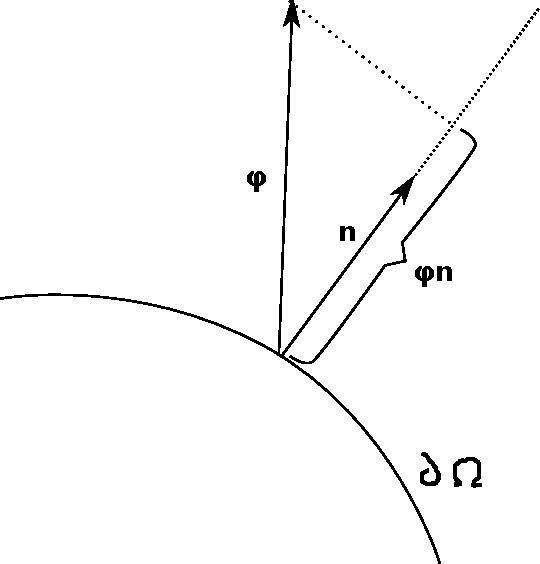
\includegraphics[width=8cm]{flux}
\caption{\label{fig:flux} The component of a flux vector
$\mathbf{\phi}$ that is directed in our out of a surface
$\partial \Omega$ is given by $\mathbf{\phi} \cdot \mathbf{n}$. Note
the sign convention.}
\end{figure*}

We can now formulate a general balance law:

\begin{eqnarray}
\frac{dG}{dt} &=& S - F \\
\frac{d}{dt} \int_\Omega g(t) dv &=& \int_\Omega s(t) dv -
\oint_{\partial \Omega} (g \mathbf{v} + \phi) \mathbf{n} \cdot da
\end{eqnarray}
Because we chose $\Omega$ such that it is a fixed volume in space,
i.e. $\Omega \ne \mathrm{fct}(t)$, the time derivative can be carried
inside the integral. A further simplification is reached by invoking
Gauss' Theorem: 

\begin{equation}
\oint_{\partial \Omega} (g \mathbf{v} + \phi) \mathbf{n} \cdot da =
\int_\Omega \nabla \cdot (g \mathbf{v} + \phi) dv
\end{equation}

A general balance law is thus

\begin{equation}
\int_\Omega \pder{g}{t} dv = \int_\Omega s(t) dv - \int_\Omega \nabla
\cdot (g \mathbf{v} + \phi) dv
\end{equation}
When we derived this law, we made no assumptions about the shape and
size of $\Omega$. In particular, we can make it infinitely small. This
integral form of the balance law then reduces to its local form

\begin{equation}
\pder{g}{t} = s(t) - (g v_i + \phi_i)_{,i} 
\end{equation}
All that remains now is to identify the relevant terms for $g$, $s$,
and $phi$.

\subsection{Conservation of mass}

In the case of mass we have $g = \rho$, $s = 0$, and $\phi = 0$. This
gives us the mass conservation law 

\begin{equation}
\pder{\rho}{t} = - \nabla \cdot (\rho \mathbf{v})
\end{equation}
This equation is greatly simplified by the fact that the density of
ice is constant; ice is a so-called \emph{incompressible} material:

\begin{equation} \label{eq:mass}
\nabla \cdot \mathbf{v} = v_{i,i} = 0
\end{equation}

\subsection{Conservation of momentum}

Momentum is a vector quantity (or first rank tensor). Its density is
given by $g = \rho \mathbf{v}$. There is a supply of momentum within
any given volume, namely that of gravity: $s = \rho \mathbf{g}$. (Apologies for
the double-meaning of $g$). There is also a surface boundary flux of
momentum into $\Omega$, which is provided by surface stresses. Think
of Newton's Second Law: Forces (stresses) are a source of momentum.

The flux term is then $\phi = -\mathbf{t}$, i.e. the Cauchy stress
tensor. Note the negative sign and the fact that $\phi$ is now a
second rank tensor. This produces a momentum balance of 

\begin{equation} \label{eq:momentum1}
\pder{\rho v_i}{t} = - (\rho v_iv_j)_{,j} + t_{ij,j} + \rho g_i
\end{equation}
Using the product rule: 

\begin{equation}
(v_iv_j)_{,j} = v_{i,j}v_j + v_iv_{j,j}
\end{equation}
The second term vanishes due to incompressibility (eqn. \ref{eq:mass})
and we are left with:

\begin{equation}
\pder{\rho v_i}{t} + \rho v_{i,j}v_j = t_{ij,j} + \rho g_i
\end{equation}
The left hand side is often written as 

\begin{equation} \label{eq:momentum}
\frac{d (\rho v_i)}{dt} = \pder{\rho v_i}{t} + \rho v_{i,j}v_j
\end{equation}
The symbol $\frac{d}{dt}$ denotes the \emph{total derivative}. It is
instructive to think about this in general terms: the change of a
quantity at one point is due to changes in time at that location
($\pder{}{t}$) plus whatever is carried there from 'upstream', which
is a product of the velocity with the gradient of the quantity.

In glaciology we simplify eqn. \ref{eq:momentum} further by neglecting
accelerations. Using typical numbers for ice flow (even very fast
flow), it can be shown that $\frac{d \rho \mathbf{v}}{dt}$ is always
much smaller than the other terms in eqn. \ref{eq:momentum}. This
approximation is known as \emph{Stokes Flow} and is typical for
creeping media. We now have:

\begin{equation}
t_{ij,j} + \rho g_i = 0
\end{equation}
You will sometimes encounter this equation in the following notation:

\begin{equation}
\nabla \cdot \mathbf{t} + \rho \mathbf{g} = 0
\end{equation}

\section{Conservation of angular momentum}

Conservation of angular momentum results in a complicated expression
that can be greatly simplified to yield

\begin{equation}
t_{ij} = t_{ji}
\end{equation}
An intuitive way of illustrating this is figure \ref{fig:angular}. If
the stress tensor were not symmetric, a net torque would result that
would lead to angular acceleration.

\begin{figure*}
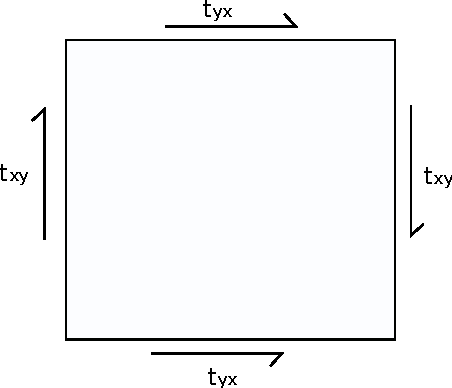
\includegraphics[width=8cm]{rotation}
\caption{\label{fig:angular} If $t_{ij} \ne t_{ji}$ a net torque and
  angular acceleration would result.}
\end{figure*}

A symmetric stress tensor has the interesting property that there is
always an orthogonal transformation that diagonalizes the tensor. In
other words, one can always find an appropriately oriented coordinate
system in which no shear stresses occur. The stresses along the main
axes of such a coordinate system are known as \emph{principal
  stresses}. This can be useful for finding maximum tensional
stresses, which determine the direction of crevassing.

\section{Conservation of energy}

The energy density is given by

\begin{equation}
g = \rho (u + \frac{v^2}{2})
\end{equation}
The first term is the inner energy, while the second one is the
kinetic energy. There is a supply of energy, which is the given by the
work done by gravity:

\begin{equation}
s=g_i v_i
\end{equation}
Finally, there are two flux terms, one is the heat flux $\mathbf{q}$,
the other one is the frictional heat due to stresses (i.e. the work
done by the stresses):

\begin{equation}
\phi_i = q_i - t_{ij} v_j
\end{equation}
Note the opposite signs: A positive heat flux implies that heat is
carried away from our sample volume, while a positive work term for
the surface stresses results in heat supplied to the sample volume. 

We thus obtain an energy balance equation

\begin{equation}
\pder{}{t} \left[ \rho \left( u + \frac{v^2}{2} \right) \right] = -
\left[ \rho \left( u + \frac{v^2}{2} \right) v_i \right]_{,i} -
q_{i,i} + (t_{ij}v_j)_{,i} + \rho g_i v_i
\end{equation}
We note, using the momentum balance (eqn. \ref{eq:momentum})
multiplied with $v_i$ that

\begin{equation}
\pder{}{t} \left[ \rho \frac{v^2}{2} \right] +
\left[ \rho \frac{v^2}{2} v_i \right]_{,i} = v_i \frac{d v_i}{dt} =
t_{ij,j}v_i + \rho g_i v_i 
\end{equation}
Note that this holds even without the Stokes approximation. We can use
the product rule to get

\begin{equation}
(t_{ij}v_j)_{,i} = t_{ij,i}v_j + t_{ij}v_{j,i} = t_{ij,j}v_i +
  t_{ij}v_{i,j}
\end{equation}
The second equality follows from the symmetry of $t_{ij}$. We also
note that $t_{ij}v_{i,j} = t_{ij}v_{j,i}$, so that

\begin{equation}
t_{ij}D_{ij} = 1/2(t_{ij}v_{i,j} + t_{ij}v_{j,i})
\end{equation}
where $D_{ij} = 1/2 (v_{i,j} + v_{j,i})$ is the strain rate tensor.

This leaves us with the following equation for energy conservation. 

\begin{equation}
\rho \frac{du}{dt} = - q_{i,i} + t_{ij}D_{ij}
\end{equation}
or

\begin{equation}
\rho \frac{du}{dt} = - \nabla \cdot \mathbf{q} + \Tr (\mathbf{tD})
\end{equation}

\section{Summary of conservation equations}

We can now summarize what we have learned from the conservation of
mass, linear and angular momentum, and energy for an incompressible
Stokes fluid. We present the equations in comma notation with Einstein
summation

\begin{eqnarray}
v_{i,i} &=& 0 \\
t_{ij,j} + \rho g_i &=& 0 \\
\rho \frac{du}{dt} + q_{i,i} - t_{ij}D_{ij} &=& 0
\end{eqnarray}
as well as the, perhaps, more familiar form

\begin{eqnarray}
\nabla \cdot \mathbf{v} &=& 0 \\
\nabla \cdot \mathbf{t} + \rho \mathbf{g} &=& 0 \\
\rho \frac{du}{dt} + \nabla \cdot \mathbf{q} - \mathrm{tr}
(\mathbf{t}\mathbf{D})  &=& 0
\end{eqnarray}
These present a total of 5 equations. Unfortunately, we are left with
13 unknowns, so additional equations are needed. These are equations
that describe the material behavior of ice.

\section{Constitutive relations}

\subsection{Viscous flow}

Stressed ice can have a variety of responses, depending on the
magnitude of stress and the time scales involved. Possible responses
involve brittle fracture, elastic recoverable deformation, and viscous
(non-recoverable) deformation. We will restrict our considerations to
viscous deformation.

It has been found experimentally that the application of a shear
stress $\tau$ will result in deformation

\begin{equation} \label{eq:glen}
\eps = A\tau^n
\end{equation}
where $\eps$ is the strain rate, $A$ is a flow-rate factor (which is
strongly temperature dependent), and $n$ is an exponent, often assumed
to be 3. This is known as a \emph{Glen-Steinemann} flow law among
glaciologists, but it turns out to be quite common for describing the
deformation of other solids, such as metals. The relation is non-linear, the ice gets
softer at higher stresses. It is also common to write this in terms of
viscosity $\eta$:

\begin{equation}
\eps = \frac{1}{2\eta}\tau
\end{equation}
For ice, the viscosity can then be written as

\begin{equation}
\eta = \frac{1}{2} A \tau^{n-1}
\end{equation}
This clearly shows that the viscosity is stress dependent, and becomes
lower at higher stresses. It also shows the peculiarity of infinite
viscosities at zero stresses. There are good theoretical and
experimental reasons why this should not be so, and $\eta$ is often
modified to account for that.

Eqn. \ref{eq:glen} relates one stress component to one strain rate
component. But the law can be generalized to account for the full
stress state as given by the stress tensor. To do this requires the
realization, however, that a uniform pressure cannot lead to
deformation in an incompressible material. We therefore have to define
a new tensor, called the \emph{deviatoric stress tensor}
$\mathbf{t}'$, that indicates the departure from a mean pressure $p$:

\begin{equation}
t_{ij} = \frac{1}{3} t_{kk}\delta_{ij} + t'_{ij} = -p \delta_{ij} +
t'_{ij}
\end{equation}
where $\delta_{ij}$ is the \emph{Kronecker symbol}. Its value is 1 if
$i=j$, and 0 otherwise. We have now introduced a new variable, the
pressure $p = 1/3 t_{kk}$. The deviatoric stress tensor is the
relevant quantity for ice deformation, and a possible generalization
for eqn. \ref{eq:glen} is the \emph{Glen-Nye} flow law:

\begin{equation} \label{eq:glennye}
D_{ij} = A(T) \mathrm{II}_{t'}^\frac{n-1}{2} t'_{ij}
\end{equation}
$\mathrm{II}_{t'}$ is the second invariant of the stress deviator (in
older literature also known as the octahedral stress):

\begin{equation}
\mathrm{II}_\mathbf{t'} = \frac{1}{2} \left( \mathrm{tr}( \mathbf{t'})
- (\mathrm{tr}\mathbf{t'})^2 \right) = \frac{1}{2}
(\mathrm{tr}\mathbf{t'})^2 
\end{equation}
Note, that $t'_{kk}$ and $D_{kk}$ both vanish, i.e. both tensors are
traceless. 

It is an easy exercise to show that eqn. \ref{eq:glennye} reduces to
eqn. \ref{eq:glen} in the presence of only one stress component. 

The flow rate factor $A$ is strongly dependent on temperature via an
\emph{Arrhenius relationship}:

\begin{equation}
A(T) = A_0 e^\frac{-Q}{kT}
\end{equation}
where $Q$ is an activation energy, and $k$ is the Boltzmann
constant. The value of $Q$ must be determined experimentally, and it
appears to change value for temperatures greater than \cels{-10}.

Note that many glaciers are at or very close to the pressure-dependent
melting point, so that the temperature is known. In that case, the
mass and momentum balance together with the flow law now form 10
equations for the 10 unknowns (3 velocity components, pressure, and 6
deviatoric stress components). With the appropriate boundary
conditions we now have a solvable set of equations. It is common to
invert equation \ref{eq:glennye} and then replace the stress tensor in
the momentum balance. This leads to the \emph{Navier-Stokes equations}
for non-linear creeping flow.

Also note that there is a fundamental difference between the flow law
discussed in this section and the conservation laws in the previous
section. The conservation laws are based on fundamental physics. The
flow law is based on a series of experiments and some theory. For
example, one has to determine experimentally whether the third
invariant should also enter eqn. \ref{eq:glennye}, or what the values
of $A_0$, $Q$, and $n$ are. There are also other dependencies for $A$,
such as grain size, dust content, water content, etc. If your
carefully designed experiment shows a discrepancy with one of the
conservation laws, you should be worried about the design of your
experiment. Should it show a discrepency with the flow law, you might
have good reason to be worried about the flow law. 

\subsection{Cold ice}

In cold ice, temperature enters as an additional variable. The
additional equation to be solved is the energy equation. But it is
again necessary to introduce two material relationships, one for the
inner energy $u$ and one for the heat flow $\mathbf{q}$. 

\begin{equation}
u = C_p T
\end{equation}
defines the specific heat $C_p$, which is a measure of how much heat
is needed to raise the temperature of a material by a certain
temperature. Heat flow can be written in terms of \emph{Fourier's
  Law}:

\begin{equation}
q_i = -k T_{,i}
\end{equation}
where $k$ is the thermal conductivity. This reduces the energy
equation to one in temperature only: 

\begin{equation}
\rho \frac{d}{dt} (C_pT) - (k T_{,i})_{,i} - t_{ij}D_{ij} = 0
\end{equation}

\section{Boundary conditions}

\subsection{Base of the ice}

There are several possible boundary conditions for the base of
the ice. Generally, this is one of the most difficult topics of
glaciology, as the base of the ice is not very amenable to
observation.

For a frozen base, the boundary conditions are (seemingly) simple:

\begin{equation}
\mathbf{v}|_{z=z_{bed}} = 0
\end{equation}
There is observational evidence for non-zero basal motion at a frozen
bed, which is almost entirely ignored in the modeling world, because
it remains well within other uncertainties.

In the case of a base at the melting point we first have to make sure
that the bed-normal velocity matches the melt rate $\dot{m}$:

\begin{equation}
v_i n_i = \dot{m}
\end{equation} 
where $\mathbf{n}$ is the unit normal vector to the bed. 

There are a variety of possible laws for basal motion. Most of them
require a knowledge of the bed-parallel stress. If $\mathbf{t}$ is the
stress tensor, then $\mathbf{t} \mathbf{n}$ is the stress on a plane
with surface normal $\mathbf{n}$. The bed-perpendicular component is
then 

\begin{equation}
(\mathbf{t} \mathbf{n}) \cdot \mathbf{n} = t_{ij}n_jn_i =  \mathbf{n}
  \mathbf{t} \mathbf{n}
\end{equation}
and the bed-parallel component therefore

\begin{equation}
\mathbf{t} \mathbf{n} - (\mathbf{n} \mathbf{t} \mathbf{n}) \mathbf{n}
\end{equation}
A common sliding law that has some theoretical justification is

\begin{equation}
\mathbf{v} = C \tau_b = C ( \mathbf{t} \mathbf{n} - (\mathbf{n}
  \mathbf{t} \mathbf{n}) \mathbf{n} )
\end{equation}
where $C$ can be a function of bed-roughness and water pressure.

If ice is underlain by till, theoretical and experimental evidence
suggests a plastic boundary condition:

\begin{eqnarray}
v_i = 0 &\mathrm{if} \, \tau_b < \tau_\mathrm{yield} \\
\tau_b = \tau_\mathrm{yield}  &\mathrm{otherwise}
\end{eqnarray}
$\tau_\mathrm{yield}$ is a till yield strength. Subglacial till does
not deform if it the applied stress is below the yield strength. Once
the yield strength is reached, the sediment can deform at any
rate. This is the characteristics of a friction law, or a perfectly
plastic material. The yield strength depends on the difference between
the pressure of the ice and the basal water pressure, as well as
material properties of the till (given by a till friction angle).

If temperature is also modelled, it is common to prescribe the
geothermal heat flux at the base of the ice, and using any excess heat
for basal melt. Things get more complicated, because ice, upon
reaching the melting point, becomes a mixture of liquid water and ice,
and needs to be treated in proper mixture theory (see lecture by
A. Aschwanden). 

\subsection{Glacier surface}

The glacier surface is subject to the atmospheric pressure

\begin{equation}
\mathbf{n} \mathbf{t} \mathbf{n} = -p_{atm}
\end{equation}

A second condition describes the effects of climate
(ablation/accumulation). It is necessary to recognize that the surface
of a glacier is not a \emph{material surface}. That is, a given set of
ice particles that constitute the surface of the ice at time $t$,
will, generally, not do so at any other times. This is because they
will either be buried by additional accumulation, or melted. Also, the
surface of the ice can move and does not need to be constant in
time. The boundary condition is:

\begin{equation}
\frac{dz}{dt}|_{z=z_\mathrm{surf}(t)} = a + w
\end{equation}
where $w$ is the vertical velocity component and $a$ is the
accumulation/ablation function, which describes the amount of ice
added or removed per unit time.

It is interesting to note that this is the only place where time
occurs explicitly. The ice flow equations are \emph{steady state
  equations} due to the Stokes approximation. The only time dependence
enters through the surface kinematic equation.

There is a second, hidden, possible time-dependence in the basal
boundary condition due to the variability of basal water pressure.

\subsection{Calving glaciers}

A third type of boundary condition can arise where ice meets water
(either ocean or lake). There is no generally agreed on calving rule
that describes the process well. This is an important topic in
glaciology, as many of the large observed changes in glaciers
originate at the ice-water interface.

\end{document}
